\documentclass[10pt,xcolor=dvipsnames,t,headinclude,headsepline=1.5cm,usepdftitle=false]{beamer}

\usepackage{framed}
\usepackage{setspace}
\usepackage{color}
\usepackage{amsmath}
\usepackage{booktabs}
\usepackage{bm}
% \usepackage{Sweave}
\usepackage{graphicx}
\usepackage{centernot}
% \usepackage{commath}
\usepackage{epstopdf}
\usepackage{caption}
\usepackage{pifont} % Symbols
\usepackage{makecell} % for line breaks in tables
\usepackage{array}
\usepackage{hyperref}
\usepackage{appendixnumberbeamer} % for \appendix, starting page counting anew from 1 for the appendix
\usepackage{multirow}
\usepackage{tabularx}

% New tabular column types
\newcolumntype{Z}{>{\centering\arraybackslash}X} % centered tabularx columns
\newcolumntype{P}[1]{>{\centering\arraybackslash}p{#1}} % like p, just centered
\newcolumntype{M}[1]{>{\centering\arraybackslash}m{#1}} % M vertically centers the content


% Theme
\usetheme{Boadilla}
\usecolortheme[named=MidnightBlue]{structure}
\definecolor{MidnightBlue}{rgb}{0.22,0.38,0.58} 
\usefonttheme{default}

\setbeamercolor{shadebox}{bg=MidnightBlue!20}

% Table of contents
\setcounter{tocdepth}{2}
% Prettify the section number in the table of contents
\setbeamertemplate{section in toc}{\inserttocsectionnumber.~\inserttocsection}

\setbeamercovered{transparent=25}
\setbeamercovered{still covered={\opaqueness<1->{0}},again covered={\opaqueness<1->{10}}}
\setbeamercovered{dynamic}
%\setbeameroption{show notes on second screen=left}
%\setbeameroption{hide only notes}
%\setbeamersize{text margin left=1cm,text margin right=10pt}
\setbeamercovered{transparent}
\setbeamertemplate{frametitle continuation}{\gdef\beamer@frametitle{}}
\setbeamertemplate{footline}{\vspace{-1cm}{\line(1,0){345}}}

    \makeatletter
    \renewenvironment{thebibliography}[1]
         {%\section*{\refname}% <--- outcommented
          \@mkboth{\MakeUppercase\refname}{\MakeUppercase\refname}%
          \list{\@biblabel{\@arabic\c@enumiv}}%
               {\settowidth\labelwidth{\@biblabel{#1}}%
                \leftmargin\labelwidth
                \advance\leftmargin\labelsep
                \@openbib@code
                \usecounter{enumiv}%
                \let\p@enumiv\@empty
                \renewcommand\theenumiv{\@arabic\c@enumiv}}%
          \sloppy
          \clubpenalty4000
          \@clubpenalty \clubpenalty
          \widowpenalty4000%
          \sfcode`\.\@m}
         {\def\@noitemerr
           {\@latex@warning{Empty `thebibliography' environment}}%
          \endlist}
    \makeatother

    \makeatletter
\newbox\@backgroundblock
\newenvironment{backgroundblock}[2]{%
  \global\setbox\@backgroundblock=\vbox\bgroup%
    \unvbox\@backgroundblock%
    \vbox to0pt\bgroup\vskip#2\hbox to0pt\bgroup\hskip#1\relax%
}{\egroup\egroup\egroup}
\addtobeamertemplate{background}{\box\@backgroundblock}{}
\makeatother

% Literatureinbindung
\usepackage[backend=bibtex, %alternativ: biber
            style=authoryear,
            citestyle=authoryear,
            dashed=false] % bei mehreren Quellen von einem Autor soll immer der Autorenname wiederholt werden im Literaturverzeichnis, und nicht ab der 2.Quelle ein Dash "-" gemacht werden statt dem Autornamen
{biblatex}
\addbibresource{../bauer_references.bib}
\DefineBibliographyStrings{ngerman}{
  andothers = {{et\,al\adddot}}, % bei mehreren Autoren 'et al.' anzeigen, ansonsten wäre es 'u.a.'
}

% Do something at the beginning of a section
% \AtBeginSection[]
% {
%   \begin{frame}[allowframebreaks]
% \frametitle{\large\bfseries Contents\\\vspace{-0.3cm}\hspace{0cm}{\rule{\textwidth}{0.5mm}}}\normalfont
% 
% \vspace{0.6cm}
% \hspace{0.5cm}\parbox[t]{.9\textwidth}{
%   \begin{minipage}[c][0.5\textheight]{\textwidth}
%   \tableofcontents[  currentsection,
%   sectionstyle=show/shaded,
%   subsectionstyle=show/show/hide]
% %  \vspace{2cm}
%   \end{minipage}
%     }
% \end{frame}
% }

% Do something at the beginning of a subsection
% \AtBeginSubsection[]
% {
%   \frame{
% \frametitle{\large\bfseries \insertsection\\\vspace{-0.3cm}\hspace{0cm}{\rule{\textwidth}{0.5mm}}}\normalfont
% %\hfill
% \vspace{2.8cm}
% \centering
% %\parbox[t]{.95\textwidth}{
% %  \begin{minipage}[c][0.5\textheight]{\textwidth}
%   \Large\bfseries\textcolor{MidnightBlue}{\insertsubsection}\normalfont\hspace{0.5cm}
% %  \end{minipage}
% %    }
%   }
% }

% gifs
\epstopdfDeclareGraphicsRule{.gif}{png}{.png}{convert gif:#1 png:\OutputFile}
\AppendGraphicsExtensions{.gif}

\colorlet{shadecolor}{MidnightBlue!20}

% No Figure in caption
\setbeamertemplate{caption}{\scriptsize\insertcaption\normalfont}

% Further settings
\beamertemplatenavigationsymbolsempty
\setbeamertemplate{itemize item}{$\bullet$}
\setbeamertemplate{itemize subit3em}{--}
\setbeamertemplate{enumerate items}[default]
\setlength{\abovedisplayskip}{0pt}
\setlength{\belowdisplayskip}{0pt}
\setlength{\abovedisplayshortskip}{0pt}
\setlength{\belowdisplayshortskip}{0pt}

% Header customization
\setbeamerfont{frametitle}{size = \large, series = \bfseries}

% ----- Newcommands
% Colors
\newcommand{\red}[1]{\textcolor{red}{#1}}
\newcommand{\blue}[1]{\textcolor{MidnightBlue}{#1}}
\newcommand{\bluebf}[1]{\textbf{\textcolor{MidnightBlue}{#1}}}
\newcommand{\darkgray}[1]{\textcolor{darkgray}{#1}}
\newcommand{\darkgraybf}[1]{\textbf{\textcolor{darkgray}{#1}}}
\newcommand{\shade}[1]{\textcolor{MidnightBlue!70}{#1}}
\newcommand{\shadesmall}[1]{{\footnotesize \textcolor{MidnightBlue!70}{#1}}}
\newcommand{\gray}[1]{\textcolor{gray!70}{#1}}
\newcommand{\graysmall}[1]{{\footnotesize \textcolor{gray!70}{#1}}}
% LMU colors
\definecolor{LMUgreen}{RGB}{0, 148, 64}		% #fce94f
\newcommand{\LMU}[1]{\textcolor{LMUgreen}{#1}}
\newcommand{\LMUbf}[1]{\textbf{\textcolor{LMUgreen}{#1}}}
\definecolor{LMUdarkgray}{RGB}{127, 127, 127}		% #fce94f
\newcommand{\LMUdarkgray}[1]{\textcolor{LMUdarkgray}{#1}}
\newcommand{\LMUdarkgraybf}[1]{\textbf{\textcolor{LMUdarkgray}{#1}}}
\definecolor{LMUlightgray}{RGB}{192, 192, 192}		% #fce94f
\newcommand{\LMUlightgray}[1]{\textcolor{LMUlightgray}{#1}}

% Individual frametitle
\newcommand{\ft}[1]{\frametitle{#1 \\ \vspace{-0.3cm}\hspace{0cm}{\rule{\textwidth}{0.5mm}}}}


% ----- Further settings
% Special packages
\usepackage{animate} % for including .gifs
\usepackage{colortbl} % for coloring \hline's in tabulars
\usepackage[overlay]{textpos} % free positioning of (background) images
\usepackage{graphbox} % vertically align images in a line
\usepackage{animate} % include gifs
\usepackage{array} % for vertical centering in table cells
% Color links
\hypersetup{
  colorlinks=true,
  urlcolor=RoyalBlue,
  linkcolor=RoyalBlue
}
% Code chunks
\usepackage{listings}
\lstset{ 
  language=R,                     % the language of the code
  basicstyle=\scriptsize\ttfamily, % the size of the fonts that are used for the code
  numbers=none,                   % where to put the line-numbers (z.B. 'numbers=left')
  numberstyle=\footnotesize\color{Blue},  % the style that is used for the line-numbers
  stepnumber=1,                   % the step between two line-numbers. If it's 1, each line will be numbered
  numbersep=5pt,                  % how far the line-numbers are from the code
  backgroundcolor=\color{gray!3},  % choose the background color. You must add \usepackage{color}
  showspaces=false,               % show spaces adding particular underscores
  showstringspaces=false,         % underline spaces within strings
  showtabs=false,                 % show tabs within strings adding particular underscores
  frame=single,                   % adds a frame around the code (z.B. 'frame=single')
  rulecolor=\color{black},        % if not set, the frame-color may be changed on line-breaks within not-black text (e.g. commens (green here))
  xleftmargin=0cm,
  tabsize=2,                      % sets default tabsize to 2 spaces
  captionpos=b,                   % sets the caption-position to bottom
  breaklines=true,                % sets automatic line breaking
  breakatwhitespace=false,        % sets if automatic breaks should only happen at whitespace
  keywordstyle=\color{Black},      % keyword style (z.B. 'RoyalBlue')
  commentstyle=\color{Green},   % comment style
  stringstyle=\color{Green}      % string literal style
}
% Footer
\setbeamertemplate{footline}{\colorbox{MidnightBlue}{\textcolor{white}{\quad Alexander Bauer \hspace{10.3cm}\insertframenumber \ / \inserttotalframenumber \hspace{2cm}}}
\beamertemplatenavigationsymbolsempty
}
% Titlepage
\title[Bauer_DAGStat]{\ \\[0.5cm] {\large \bf KOALA: A new paradigm for election coverage} \\[0.2cm] {\normalsize An opinion poll based ``now-cast'' of probabilities of events in \\ multi-party electoral systems \\[0.25cm]}}
\subtitle[Kurzform]{
\vspace{-0.3cm}
\rule{0.85\textwidth}{0.3mm} \\[0.45cm]
{\normalsize Alexander Bauer} \\
{\scriptsize Statistical Consulting Unit StaBLab, LMU Munich} \\[0.25cm]
{\footnotesize DAGStat \textbar \ March 20, 2019 \textbar \ Munich}
}
\author[A. Bauer]{\vspace{-1cm}
\normalfont}
\date{}
% ----- End of settings


\begin{document}

\frame{
\vspace{1cm}
\titlepage
}

% Second titlepage
\title[Bauer_DAGStat]{\\[11px]

\includegraphics[width=0.35\textwidth]{figures/koala} \\[0.1cm]}
\subtitle[Kurzform]{
\vspace{-0.3cm}
\rule{0.85\textwidth}{0.3mm} \\[0.45cm]
{\normalsize Alexander Bauer} \\
{\scriptsize Statistical Consulting Unit StaBLab, LMU Munich} \\[0.25cm]
{\footnotesize DAGStat \textbar \ March 20, 2019 \textbar \ Munich}
}
\author[A. Bauer]{\vspace{-1cm}
\normalfont}
\date{}

\addtocounter{framenumber}{-1}
\frame{
\vspace{1cm}
\titlepage
}

% Third titlepage
\title[Bauer_DAGStat]{\\[11px]

\includegraphics[width=0.35\textwidth]{figures/koala} \\[0.1cm]}
\subtitle[Kurzform]{
\vspace{-0.3cm}
\rule{0.85\textwidth}{0.3mm} \\[0.45cm]
}
\author[A. Bauer]{\vspace{-1cm}
\normalfont}
\date{}

\addtocounter{framenumber}{-1}
\frame{
\vspace{-11px}
\titlepage
\vspace{-95px}
\hspace{17px}
\begin{tabular}{ll}
\bluebf{\footnotesize Collaborators} & \\
\blue{\footnotesize Dr. Andreas Bender} & \blue{\footnotesize Nuffield Department of Clinical Medicine,} \\
& \blue{\footnotesize University of Oxford, United Kingdom} \\
\blue{\footnotesize Dr. Andr\'e Klima} & \blue{\footnotesize StaBLab, LMU Munich} \\
\blue{\footnotesize Prof. Dr. Helmut K\"uchenhoff} & \blue{\footnotesize StaBLab, LMU Munich} \\
\end{tabular}
}

% ----- Outline
\frame{\ft{Outline}
  \tableofcontents[subsectionstyle=show/show/hide]
}
\addtocounter{framenumber}{-1}


% ----- Motivation
\section{Motivation}
\frame{\ft{Outline}
  \tableofcontents[currentsection, subsectionstyle=show/show/hide]
}

\frame{\ft{\large{\blue{\ding{202}}} Motivation}
\begin{center}
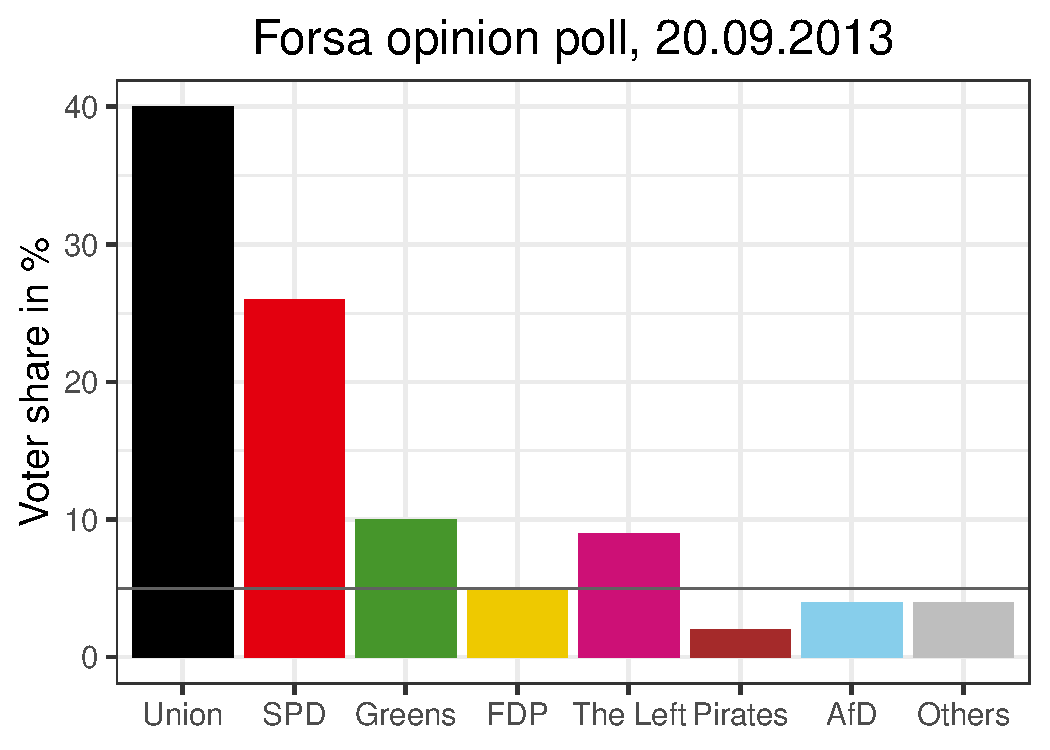
\includegraphics[width=0.5\textwidth]{figures/motivation_forsa_130920}
\end{center}
\bigskip
\textbf{Questions of interest}
\begin{itemize}
  \item Which parties will pass the $5\%$ hurdle and enter the parliament?
  \item Which parties will form the governing coalition?
%  \item Which party will have the third largest share of votes?
\end{itemize}}

\addtocounter{framenumber}{-1}
\frame{\ft{\large{\blue{\ding{202}}} Motivation}
\textbf{Reported voter shares} {\footnotesize (Forsa, last pre-election poll 2013)} \\[0.37cm]
\begin{center}
{\footnotesize
\begin{tabular}{cccccccc}
\toprule[0.09 em]
Union & \textcolor{black!40}{SPD} & \textcolor{black!40}{Greens} & FDP &
\textcolor{black!40}{The Left} & \textcolor{black!40}{Pirates} & 
\textcolor{black!40}{AfD} & \textcolor{black!40}{Others} \\
\midrule
40\% & \textcolor{black!40}{26\%} & \textcolor{black!40}{10\%} & 5\% &
\textcolor{black!40}{9\%} & \textcolor{black!40}{2\%} & 
\textcolor{black!40}{4\%} & \textcolor{black!40}{5\%} \\
\bottomrule[0.09 em]
\end{tabular}
}
\end{center}
\medskip
\pause
\textbf{Redistributed voter shares} {\footnotesize (based on $5\%$ hurdle)} \\[0.37cm]
\begin{center}
{\footnotesize
\begin{tabular}{cccccccc}
\toprule[0.09 em]
Union & \textcolor{black!40}{SPD} & \textcolor{black!40}{Greens} & FDP &
\textcolor{black!40}{The Left} & \textcolor{black!40}{Pirates} & 
\textcolor{black!40}{AfD} & \textcolor{black!40}{Others} \\
\midrule
44.44\% & \textcolor{black!40}{28.89\%} & \textcolor{black!40}{11.11\%} & 5.56\% &
\textcolor{black!40}{10.00\%} & \textcolor{black!40}{-} & 
\textcolor{black!40}{-} & \textcolor{black!40}{-} \\
\bottomrule[0.09 em]
\end{tabular}
}
\end{center}
\bigskip
\pause
\begin{itemize}
  \item Union-FDP have a joint seat share of exactly $50\%$
  \pause
  \item Stating that Union-FDP would thus miss a joint majority would neglect sample uncertainty
\end{itemize}
}

\frame{\ft{\large{\blue{\ding{202}}} Motivation}
\vspace{30px}
\bluebf{We aim to do} \textbf{now-casting} \\[0.1cm]
We communicate sample uncertainty in a more natural way
by calculating \\ \textbf{event probabilities} that fully reflect sample uncertainty.
\\[1.5cm]
%\begin{itemize}
%  \item We incorporate the uncertainty as reported by the polling agencies
%  \item Potential house biases or an industry bias are not accounted for
%\end{itemize}
%\bigskip \bigskip
\pause
\bluebf{We} \redbf{do not} \bluebf{aim to do} \redbf{for-casting}
\begin{itemize}
  \item Our approach simply communicates sample uncertainty in a novel way
  \item Also, a relevant share of voters is still undecided shortly before election day (Küchenhoff et al., 2018)
\end{itemize}
}

% ----- Methods
\section{Methods}
\frame{\ft{Outline}
\tableofcontents[currentsection, subsectionstyle=show/show/hide]
}

\frame{\ft{\large{\blue{\ding{203}}} Methods}
\textbf{Estimating probabilities of events (POEs)} \\[0.1cm]
Given one opinion poll with sample size $n$:
$$
\boldsymbol{X} = (X_1,\ldots, X_P)^T \sim Multinomial(n, \theta_1,\ldots, \theta_P),
$$
with voter counts $X_j$ and the true percentage of voters $\theta_j$ per party $j$.
%\\ {\footnotesize (assuming a simple random sample, ignoring a possible bias)}
\\[0.8cm]
\pause
A \textbf{Dirichlet posterior distribution} results for $\boldsymbol{\theta} | \boldsymbol{x}$:
$$
\boldsymbol{\theta}|\mathbf{x} \sim Dirichlet(x_1 + 1/2,\ldots, x_P + 1/2),
$$
\pause
\ \\
based on an \textbf{uninformative Dirichlet prior}
% for the true party shares
(Gelman et al., 2013)
$$
\begin{aligned}
\boldsymbol{\theta} &= (\theta_1,\ldots,\theta_P)^T \sim Dirichlet(\alpha_1,\ldots,\alpha_P), \\
\text{with} &\ \ \ \ \ \ \ \ \ \ \ \ \ \ \ \alpha_1 = \ldots = \alpha_P = \frac{1}{2}.
\end{aligned}
$$
}

\frame{\ft{\large{\blue{\ding{203}}} Methods}
\textbf{Estimating probabilities of events (POEs)} \\[0.5cm]
Given the \bluebf{posterior distribution of voter shares} we can use \\ 
\textbf{Monte Carlo simulations} to estimate POEs: \\[0.1cm]
\begin{enumerate}
  \item Simulate $10\,000$ election outcomes from the posterior \\
  {\footnotesize (adding uniformly distributed random noise to account for rounding errors)}
  \item If necessary: Redistribute voter shares to get obtained seats in parliament
  \item POE $= \frac{\#\text{events}}{\text{number of simulations}}$
\end{enumerate}
\bigskip \bigskip
\pause
\textbf{Example} \\[0.1cm]
Given the Forsa poll, the coalition of Union-FDP obtained a majority of seats in
$2\,633$ of $10\,000$ simulations \\[0.2cm]
$\Rightarrow \text{POE} \approx 26\%$
}

\frame{\ft{\large{\blue{\ding{203}}} Methods}
\textbf{Visualization using ridgeline plots} (Wilke, 2017)
\\[1.1cm]
\begin{tabular}{ m{.28\textwidth} m{.7\textwidth} }
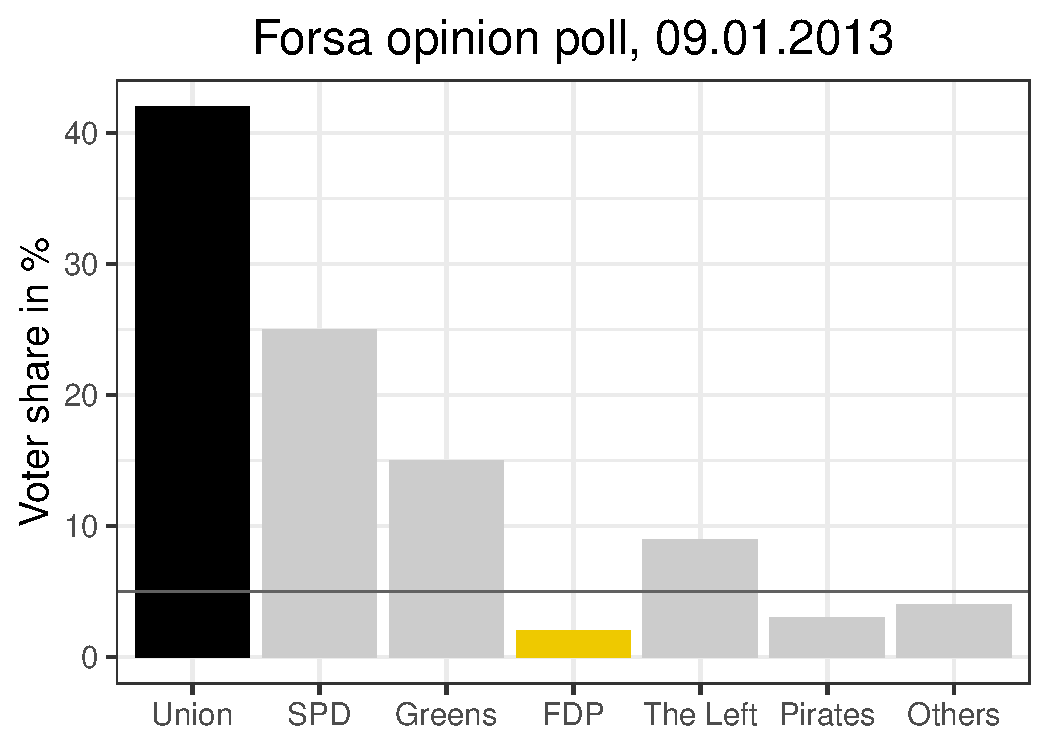
\includegraphics[width=.28\textwidth]{figures/motivation_forsa_130109_bw} &
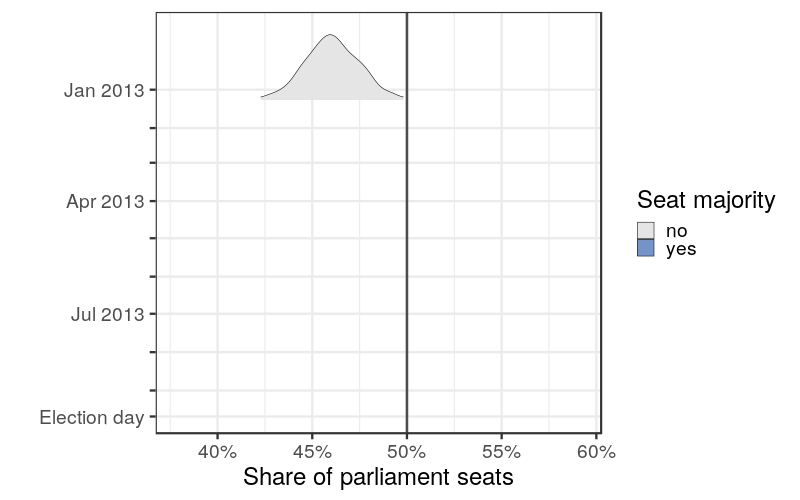
\includegraphics[width=.68\textwidth]{figures/gif/frame-0}
\end{tabular}
\vspace{-10px}
}

\addtocounter{framenumber}{-1}
\frame{\ft{\large{\blue{\ding{203}}} Methods}
\textbf{Visualization using ridgeline plots} (Wilke, 2017)
\\[1.1cm]
\begin{tabular}{ m{.28\textwidth} m{.7\textwidth} }
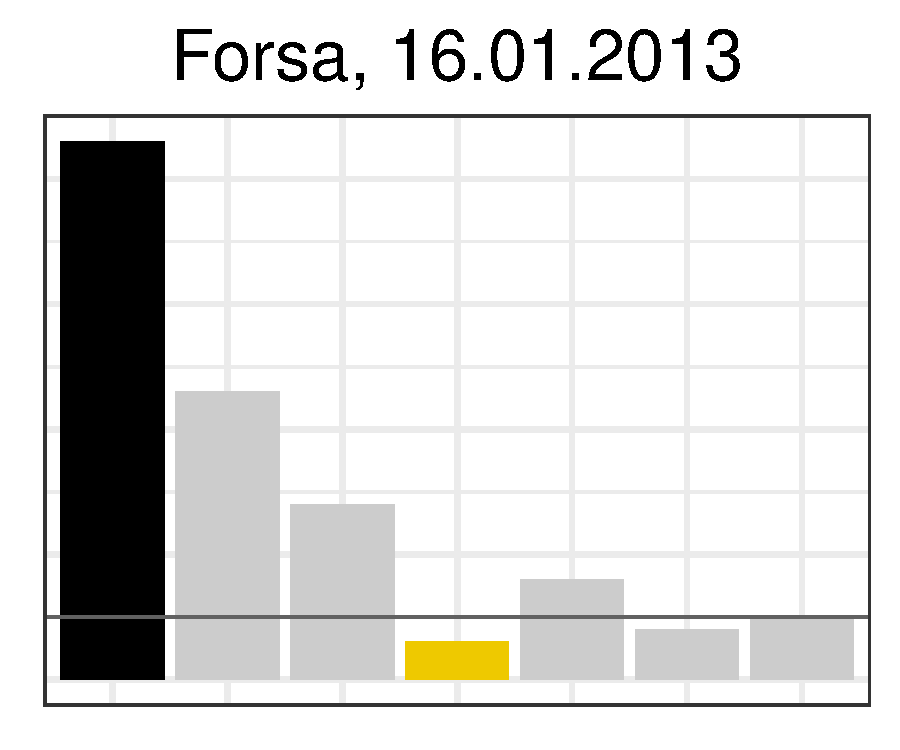
\includegraphics[width=.28\textwidth]{figures/motivation_forsa_130116_bw} &
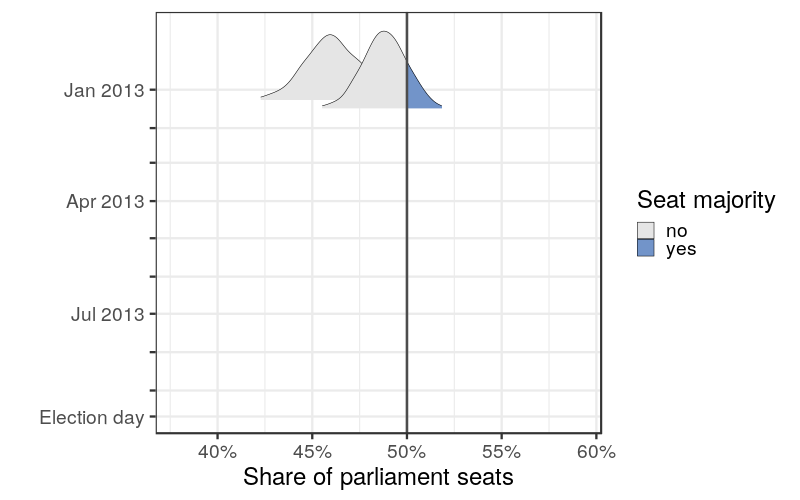
\includegraphics[width=.68\textwidth]{figures/gif/frame-1}
\end{tabular}
\vspace{-10px}
}

\addtocounter{framenumber}{-1}
\frame{\ft{\large{\blue{\ding{203}}} Methods}
\textbf{Visualization using ridgeline plots} (Wilke, 2017)
\\[1.1cm]
\begin{tabular}{ m{.28\textwidth} m{.7\textwidth} }
&
\animategraphics[width=.68\textwidth]{5}{figures/gif/frame-}{1}{11} \\
& {\footnotesize \textcolor{black!40}{I'm a .gif, click me (in Adobe Acrobat)!}} \\
\end{tabular}
\vspace{-10px}
}

\addtocounter{framenumber}{-1}
\frame{\ft{\large{\blue{\ding{203}}} Methods}
\textbf{Visualization using ridgeline plots} (Wilke, 2017)
\\[1.1cm]
\begin{tabular}{ m{.28\textwidth} m{.7\textwidth} }
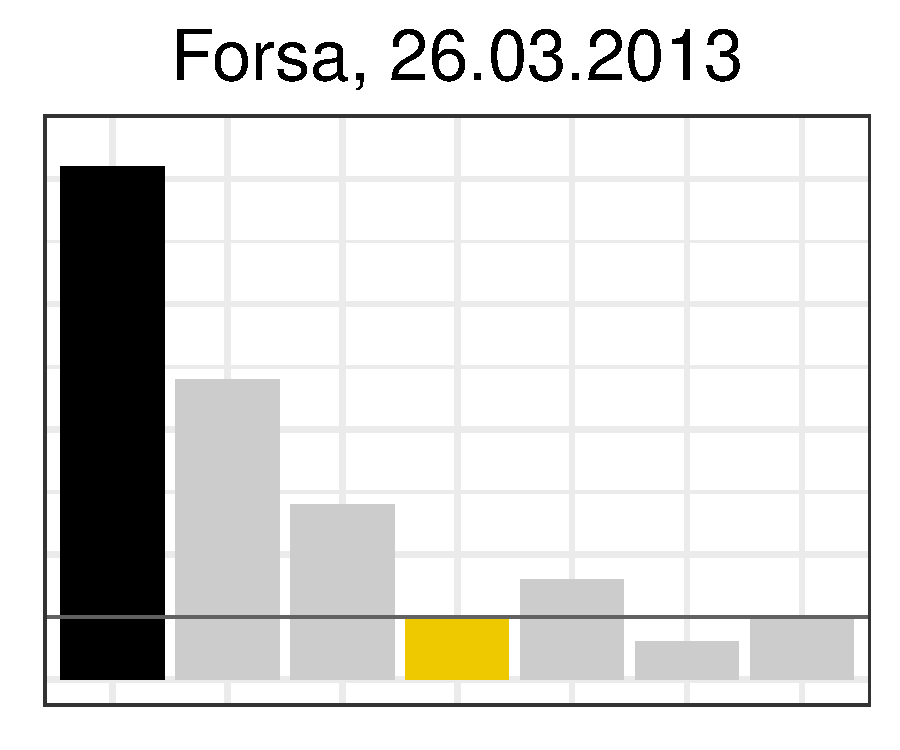
\includegraphics[width=.28\textwidth]{figures/motivation_forsa_130326_bw} &
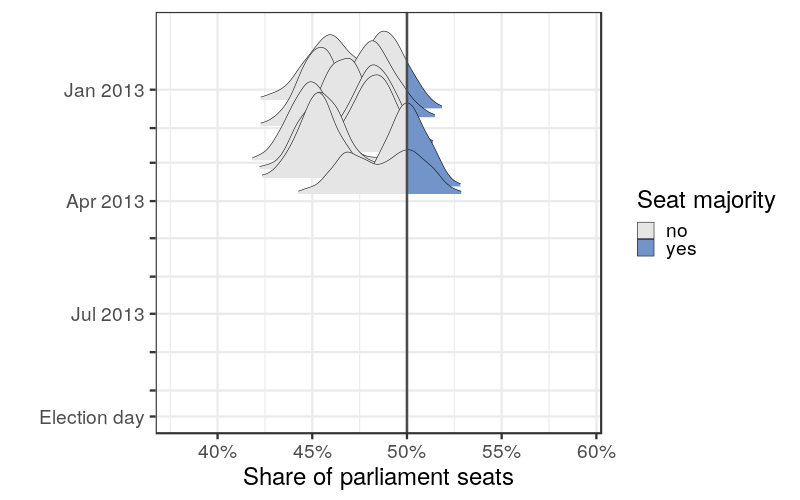
\includegraphics[width=.68\textwidth]{figures/gif/frame-11}
\end{tabular}
\vspace{-10px}
}

\addtocounter{framenumber}{-1}
\frame{\ft{\large{\blue{\ding{203}}} Methods}
\textbf{Visualization using ridgeline plots} (Wilke, 2017)
\\[1.1cm]
\begin{tabular}{ m{.28\textwidth} m{.7\textwidth} }
&
\animategraphics[width=.68\textwidth]{5}{figures/gif/frame-}{11}{37} \\
& {\footnotesize \textcolor{black!40}{I'm a .gif, click me (in Adobe Acrobat)!}} \\
\end{tabular}
\vspace{-10px}
}

\frame{\ft{\large{\blue{\ding{203}}} Methods}
\textbf{Visualization using ridgeline plots} (Wilke, 2017)
\\[1.1cm]
\begin{center}
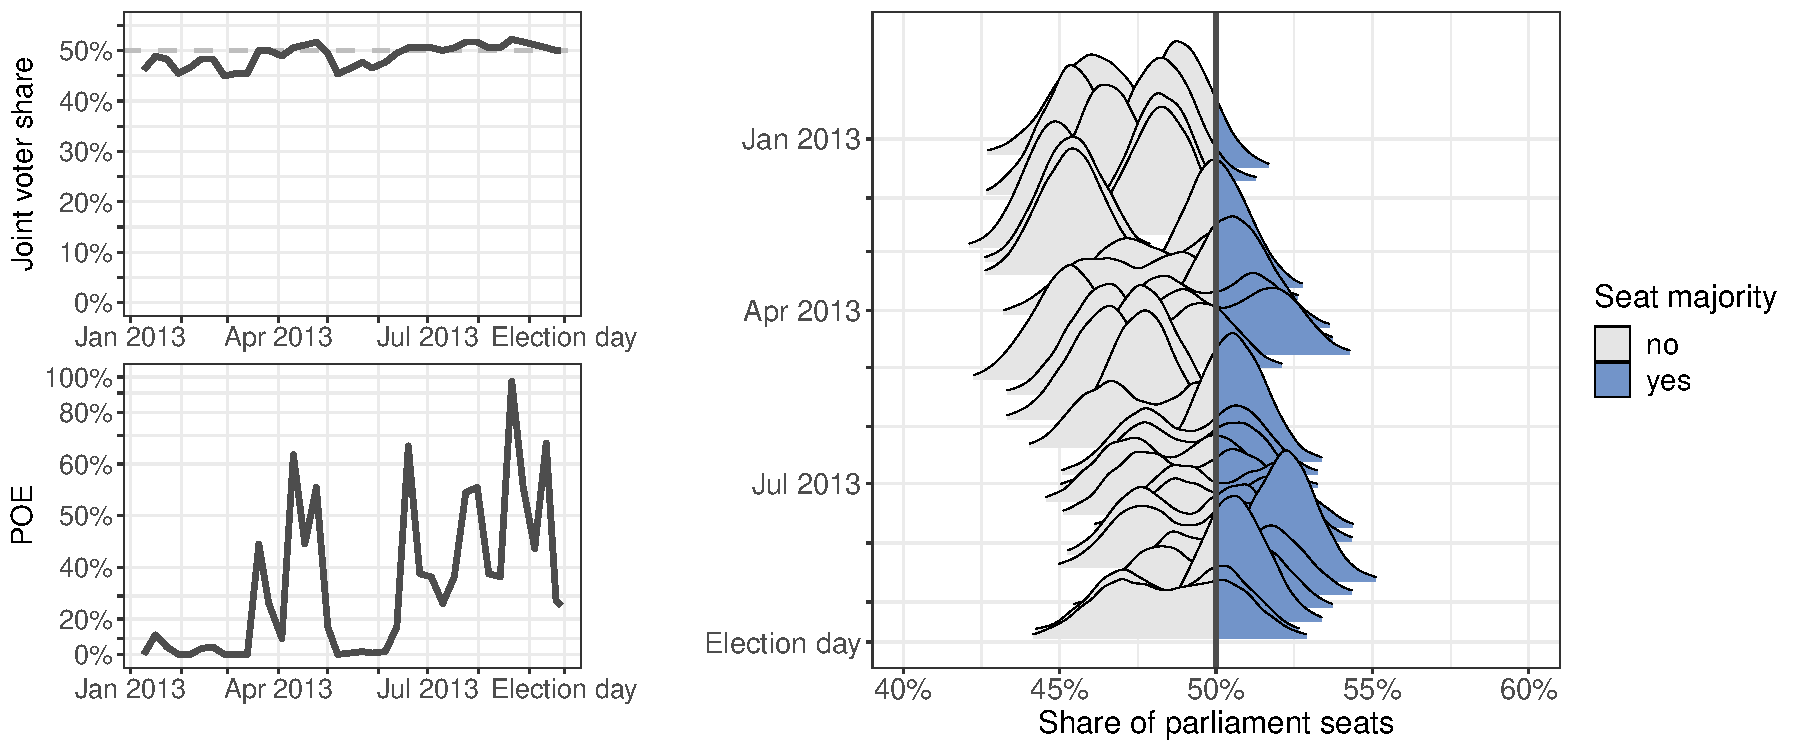
\includegraphics[width=1\textwidth]{figures/cdufdp_2013_joint}
\end{center}
}

\frame{\ft{\large{\blue{\ding{203}}} Methods}
\textbf{Pooling} \\[0.1cm]
We aggregate multiple polls to reduce sample uncertainty. \\
In case of multiple random samples:
\\[0.3cm]
$$
\left( \sum\limits_i X_{i1},\ldots, \sum\limits_i X_{iP} \right)^T
 \sim Multinomial \left( \sum\limits_i n_i,\theta_1,\ldots,\theta_P\right).
$$
\ \\[0.6cm]
We account for correlations between polling agencies by using an \\
\textbf{effective sample size} (Hanley et al., 2003).
\\[0.8cm]
\pause
\textbf{Example} \\[0.1cm]
Pooling two polls with \bluebf{$1\,500$} and \bluebf{$2\,000$} respondents
we get an effective \\ sample size of \bluebf{$n_{\text{eff}} = 2\,341$}
{\footnotesize (based on a strongest party share of $40\%$)}.
}

\frame{\ft{\large{\blue{\ding{203}}} Methods}
\textbf{Pooling} \\[0.1cm]
We aggregate multiple polls to reduce sample uncertainty. \\
In case of multiple random samples:
\\[0.3cm]
$$
\left( \sum\limits_i X_{i1},\ldots, \sum\limits_i X_{iP} \right)^T
 \sim Multinomial \left( \sum\limits_i n_i,\theta_1,\ldots,\theta_P\right).
$$
\ \\[0.6cm]
We account for correlations between polling agencies by using an \\
\textbf{effective sample size} (Hanley et al., 2003).
\\[0.8cm]
\textbf{Pooling in practice} \\[0.1cm]
\begin{itemize}
  \item We only pool surveys published in the last $14$ days
  \item We only include one survey per polling agency
\end{itemize}
}

% ----- Technical implementation
\section{Technical implementation}
\frame{\ft{Outline}
\tableofcontents[currentsection, subsectionstyle=show/show/hide]
}

\begin{frame}[fragile]
\ft{\large{\blue{\ding{204}}} Technical implementation}
\begin{textblock*}{1.25cm}(0.89\textwidth,0px)

\includegraphics[width=1\textwidth]{figures/coalitions_hex}
\end{textblock*}
\vspace{10px}
\textbf{R package \texttt{coalitions}}
\\[1cm]
\textbf{Functionality}
\begin{itemize}
  \item Scrape \href{https://www.wahlrecht.de/}{wahlrecht.de} for (new) polls
  \item Calculate pooled sample
  \item Sample from posterior distribution
  \item Redistribute votes below 5\% threshold \\[0.1cm]
and calculate parliament seats 
{\footnotesize (e.g. based on method by \href{http://www.wahlrecht.de/verfahren/rangmasszahlen.html}{Sainte-Lagu\"e-Schepers})}
  \item Calculate coalition probabilities
\end{itemize}
\bigskip
More on \href{https://github.com/adibender/coalitions/}{github.com/adibender/coalitions}
\end{frame}

%\begin{frame}[fragile]
%\ft{\large{\blue{\ding{204}}} Technical implementation}
%\begin{textblock*}{1.25cm}(0.89\textwidth,0px)
%
\includegraphics[width=1\textwidth]{figures/coalitions_hex}
%\end{textblock*}
%\vspace{10px}
%\textbf{R package \texttt{coalitions}}
%\\[0.7cm]
%\begin{lstlisting}
%> library(coalitions)
%> library(tidyverse)
%
%> surveys <- get_surveys()
%> surveys
%
%# A tibble: 7 x 2
%  pollster   surveys
%  <chr>      <list>
%1 allensbach <tibble [42 x 5]>
%2 emnid      <tibble [226 x 5]>
%3 forsa      <tibble [236 x 5]>
%...
%
%> survey <- surveys %>% unnest() %>% slice(1)
%> survey %>% get_probabilities(list(c("cdu","fdp")), nsim = 10000) %>%
%    unnest()
%# A tibble: 1 x 4
%  pollster   date       coalition probability
%  <chr>      <date>     <chr>           <dbl>
%1 allensbach 2019-02-19 cdu_fdp             0
%\end{lstlisting}
%\end{frame}

\frame{\ft{\large{\blue{\ding{204}}} Technical implementation}
\begin{textblock*}{3cm}(0.78\textwidth,0px)

\includegraphics[align=c,width=0.4\textwidth]{figures/shiny}
\ \ 

\includegraphics[align=c,width=0.28\textwidth]{figures/twitter}
\end{textblock*}
\vspace{10px}
\textbf{Web-Interface}
\\[1cm]
\textbf{Communicating the results}
\begin{enumerate}
  \item Website \href{https://koala.stat.uni-muenchen.de}{\texttt{koala.stat.uni-muenchen.de}} \\[0.1cm]
$\Rightarrow$ Automatic updates scraping data from wahlrecht.de
  \item Twitter \href{https://twitter.com/KOALA_LMU}{@KOALA\_LMU} \\[0.1cm]
$\Rightarrow$ Automatic tweets of new results
  \item Blog \href{https://koala-blog.netlify.com/portfolio/}{koala-blog.netlify.com}
\end{enumerate}
\bigskip
\pause
\textbf{Technical implementation in R}
\begin{itemize}
  \item User interface was built with the \href{http://shiny.rstudio.com/}{shiny} package
  \item Server is based on \href{https://www.rstudio.com/products/shiny/shiny-server/}{Shiny Server Open Source}
  \item Tweets are sent with the \href{https://github.com/geoffjentry/twitteR}{twitteR} package
\end{itemize}
}



% ----- Conclusion
\section{Conclusion}
\frame{\ft{Outline}
\tableofcontents[currentsection, subsectionstyle=show/show/hide]
}

\frame{\ft{\large{\blue{\ding{205}}} Conclusion}
\vspace{5px}
\begin{center}

\includegraphics[width=0.3\textwidth]{figures/koala}
\end{center}
\bigskip \medskip
\textbf{The KOALA approach}
\begin{itemize}
  \item New paradigm for opinion poll coverage
  \item Bayesian approach to now-cast POEs
  \item Sample uncertainty is reduced by pooling multiple polls
  \item Communication to the general public
  \item[]
  \item \bluebf{Keep in mind:} We calculate now-casts, not for-casts
\end{itemize}
}


% Materials
\addtocounter{framenumber}{-1}
\frame{\ft{References}
\bluebf{KOALA} \\[0.07cm]
{\footnotesize
\textbf{Bauer, A., Bender, A., Klima, A., and Küchenhoff, H. (2018)} \textcolor{darkgray}{KOALA: A new paradigm for election coverage. \textit{arXiv.org}. URL \texttt{http://arxiv.org/abs/1807.09665}.} \\[0.04cm]
\textbf{Bender, A., and Bauer, A. (2018)} \textcolor{darkgray}{coalitions: Coalition probabilities in multi-party democracies. \textit{The Journal of Open Source Software}. doi: 10.21105/joss.00606. \\ URL \texttt{http://joss.theoj.org/papers/10.21105/joss.00606}.}
} \ \\[0.5cm]
\bluebf{Methods} \\[0.07cm]
{\footnotesize
\textbf{Gelman, A. et al. (2013)} \textcolor{darkgray}{\textit{Bayesian data analysis}, volume 3. CRC press Boca Raton, FL.} \\[0.04cm]
\textbf{Hanley, J. A. et al. (2003)} \textcolor{darkgray}{Statistical analysis of correlated data using generalized estimating equations: an orientation. \textit{American journal of epidemiology}, 157(4), 364--375.} \\[0.04cm]
\textbf{Küchenhoff, H. et al. (2018)} \textcolor{darkgray}{\textit{Universitätsstudie zur Bayernwahl USBW 18 (München -- Passau -- Regensburg). Erste Ergebnisse -- Oktober 2018.} \\ URL \texttt{https://www.stablab.stat.uni-muenchen.de/lehre/pdfs/usbw18.pdf}.}
} \ \\[0.5cm]
\bluebf{Further software} \\[0.07cm]
{\footnotesize
\textbf{Chang, W. et al. (2017)} \textcolor{darkgray}{\textit{shiny: Web Application Framework for R}. \\ URL \texttt{https://CRAN.R-project.org/package=shiny}. R package version 1.0.5.} \\[0.04cm]
\textbf{Wilke, C. O. (2017)} \textcolor{darkgray}{\textit{ggridges: Ridgeline Plots in 'ggplot2'}. \\ URL \texttt{https://CRAN.R-project.org/package=ggridges}. R package version 0.4.1.} \\[0.04cm]
}
}

\end{document}